\documentclass[a4paper, 11pt]{article}
\usepackage[top=3cm, bottom=3cm, left=2cm, right=2cm]{geometry} 
\geometry{a4paper} 
\usepackage[utf8]{inputenc}
\usepackage[vietnamese]{babel}
\usepackage{xcolor}
\usepackage{sectsty}
\usepackage{textcomp}
\usepackage{graphicx} 
\usepackage{amsmath,amssymb}
\usepackage{algorithm,algcompatible}
\usepackage{caption}
\usepackage{subcaption}
\usepackage{bm}
\usepackage{tikz}
\usepackage{multirow, multicol, makecell}
\usepackage{longtable}
\usepackage{enumitem}
\setlist[itemize]{leftmargin=*}
\usepackage[pdftex,bookmarks,colorlinks,breaklinks]{hyperref}  
%\hypersetup{linkcolor=black,citecolor=black,filecolor=black,urlcolor=black} % black links, for printed output
\usepackage{memhfixc}
\usepackage{wrapfig}
\usepackage{pdfsync}  
\usepackage{fancyhdr}
\usepackage{pifont}
\usepackage{listings}
\usepackage{lstfiracode}
\lstset{style=FiraCodeStyle,basicstyle=\ttfamily,columns=fullflexible,breaklines=true,commentstyle=\color{green},
keywordstyle=\color{magenta},
numberstyle=\color{gray},
stringstyle=\color{red}}
\makeatletter
\def\lst@visiblespace{ }
\makeatother
\usepackage[export]{adjustbox}

\pagestyle{fancy}
\sloppy

\graphicspath{ {images/} }
\setlength{\headheight}{16.50983pt}
\setlength{\parindent}{0pt}

\newenvironment{vnalgorithm}[1][]
  {\begin{algorithm}[#1]
     \selectlanguage{vietnamese}%
     \floatname{algorithm}{Thuật toán}%
     \algnewcommand\INPUT{\item[\textbf{Đầu vào:}]}%
     \algnewcommand\OUTPUT{\item[\textbf{Đầu ra:}]}%
     \algnewcommand\BEGIN{\item[\textbf{begin}]} %
     \algnewcommand\DO{\textbf{ do}} %
     \algnewcommand\RETURN{\State\textbf{return }}%
     \algnewcommand\BREAK{\State\textbf{break}}%
     \algnewcommand\CONTINUE{\State\textbf{continue}}
     \algnewcommand\END{\item[\textbf{end}]}%
     % Set other language requirements
  }
  {\end{algorithm}}


\title{\textbf{Bài tập Thực hành Nhập môn Trí tuệ Nhân tạo tuần 4}}
\author{Nguyễn Lê Ngọc Duy - 20280023 - 20KDL1}
\date{}

\begin{document}
\maketitle
\hypersetup{linkcolor=black}
\tableofcontents
\clearpage

\section{Bài toán người đi du lịch - Travelling salesman problem (TSP).}

Trong các bài toán về đường đi, bài toán người đi du lịch (còn gọi tắt là TSP) là một trong những bài toán được nghiên cứu nhiều nhất. Bài toán này được đề xuất vào thế kỉ XVII bởi hai nhà toán học vương quốc Anh là Sir William Rowan Hamilton và Thomas Penyngton Kirkman, và được ghi trong cuốn giáo trình Lý thuyết đồ thị nổi tiếng của Oxford. Nó nhanh chóng trở thành bài toán khó thách thức toàn thế giới bởi độ phức tạp thuật toán tăng theo hàm số mũ (trong chuyên ngành thuật toán người ta còn gọi chúng là những bài toán NP-hard). Người ta bắt đầu thử và công bố các kết quả giải bài toán này trên máy tính từ năm 1954 (49 đỉnh), cho đến năm 2004 bài toán giải được với số đỉnh lên tới 24.978, và dự báo sẽ còn tiếp tục tăng cao nữa.

Bài toán này được đặt ra như sau: Cho một tập các thành phố và khoảng cách giữa các cặp thành phố, đồng thời giữa hai thành phố bất kì \textbf{luôn tồn tại đường đi giữa hai thành phố đó với nhau}, nhiệm vụ của chúng ta tìm một đường đi bắt đầu từ thành phố xuất phát, đi qua tất cả các thành phố đúng 1 lần và trở lại thành phố xuất phát sao cho tổng đường đi là nhỏ nhất.

Ta có thể phát biểu lại bài toán dưới đạng đồ thị như sau: Cho một đồ thị vô hướng có trọng số, giữa hai đỉnh của đồ thị luôn được nối với nhau bởi ít nhất một cạnh, hãy tìm một đường đi bắt đầu từ đỉnh xuất phát, đi qua tất cả các đỉnh của đồ thị đúng 1 lần và quay trở lại đinh xuất phát sao cho độ dài của dường đi là nhỏ nhất.

Cho đến ngày này, các nhà khoa học đã tìm ra được nhiều phương pháp để giải quyết bài toán. Trong khuôn khổ của bài báo cáo tuần này, chúng ta sẽ cùng đi sâu vào cách giải sử dụng thuật toán A*, kết hợp bởi \textbf{cây khung nhỏ nhất} (Minimum Spanning Tree - MST) và thuật heuristic \textbf{chèn gấn nhất} (Nearest Insertion).

\begin{figure}[h]
  \centering
  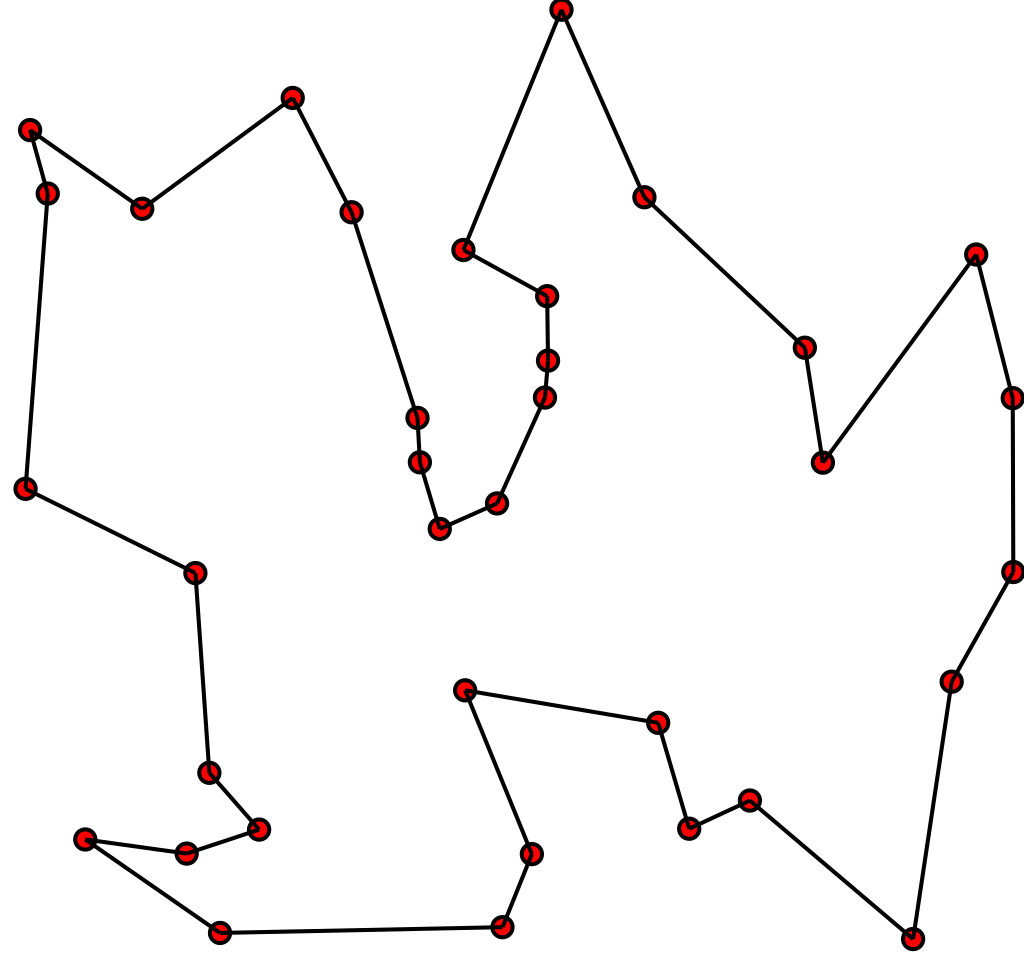
\includegraphics[width=0.5\textwidth, height=0.5\textheight,keepaspectratio]{TSP.png}
  \caption{Một lời giải cho bài toán TSP}
\end{figure}

\clearpage
\section{Cây khung nhỏ nhất (MST) - Thuật toán Prim.}
\subsection{Cây khung nhỏ nhất (MST).}
Trong lý thuyết đồ thị, \textbf{cây khung nhỏ nhất} của đồ thị có trọng số $G = (V, E)$ là một tập hợp các cạnh của đồ thị sao cho:
\begin{itemize}
  \item Tập hợp các cạnh này \textit{không chứa chu trình} và \textit{liên thông} - nghĩa là từ một đỉnh bất kỳ có thể đi tới các đỉnh khác mà chỉ dùng các cạnh trên tập hợp đó.
  \item Tổng trọng số của các cạnh trong tập hợp này là \textit{nhỏ nhất}.
\end{itemize}

\begin{figure}[h]
  \centering
  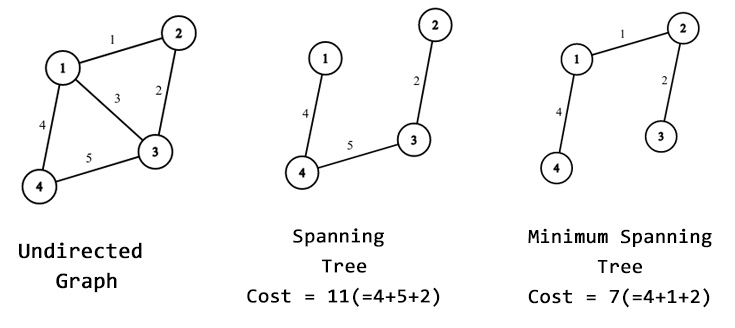
\includegraphics[width=0.75\textwidth, height=0.75\textheight,keepaspectratio]{st_mst.png}
  \caption{Minh hoạ cây khung và cây khung nhỏ nhất của đồ thị vô hướng có trọng số}
\end{figure}

Trong bài báo cáo này, chúng ta sẽ tìm hiểu một thuật toán có thể tìm được cây khung nhỏ nhất của đồ thị, đó là thuật toán Prim.

\subsection{Thuật toán Prim.}
Về mặt ý tưởng, thuật toán Prim rất giống với ý tưởng của thuật toán Dijikstra (tìm đường đi ngắn nhất trên đồ thị). Thuật toán Prim kết nạp từng đỉnh của đồ thị theo tiêu chí: đỉnh được kết nạp vào tiếp theo phải \textit{chưa được nạp} và \textit{gần nhất} với các đỉnh đã được nạp vào đò thị. Ta có thể dùng một hàng đợi ưu tiên lưu lại các cạnh có trọng số nhỏ nhất, khi đó độ phức tạp thời gian của thuật toán Prim là $O((V + E) \log V)$ vì mỗi đỉnh được thêm vào hàng đợi chỉ một lần và thao tác thêm phần tử vào hàng đợi có chi phí thời gian là hàm logarit.

Mã giả cho thuật toán Prim và hình ảnh minh hoạ thuật toán được thể hiện dưới đây.

\begin{vnalgorithm}
  \caption{Thuật toán Prim}
  \begin{algorithmic}[1]
    \INPUT Đồ thị vô hướng, liên thông, có trọng số  $G = (V, U)$
    \OUTPUT Cây khung nhỏ nhất $T$ của đồ thị $G$.
    \STATE Chọn một đỉnh bất kì $s \in G$.
    \STATE $D[s] = 0$
    \FOR {\textbf{each} $v \in V \setminus \{s\}$}
      \STATE $D[v] = \infty$
      \STATE $v.$parent = \textbf{null}
    \ENDFOR
    \STATE Khởi tạo $T = \emptyset$
    \STATE Khởi tạo hàng đợi ưu tiên $Q = (D[v], v)$ \textbf{for each} $v \in V$.
    \STATE $T.$connect$(u)$
    \WHILE {$Q$ không rỗng}
      \STATE {$u = Q.$removeMin()}
      \FOR {\textbf{each} $v \in G.$adjacent$[u]$}
        \IF{$v \in Q$ và $w(u, v) < D[v]$}
          \STATE $D[v] = w(u, v)$
          \STATE $v.$parent = $u$
          \STATE $T.$connect$(v)$
        \ENDIF
      \ENDFOR
    \ENDWHILE
  \end{algorithmic}
\end{vnalgorithm}

\begin{figure}[h]
  \centering
  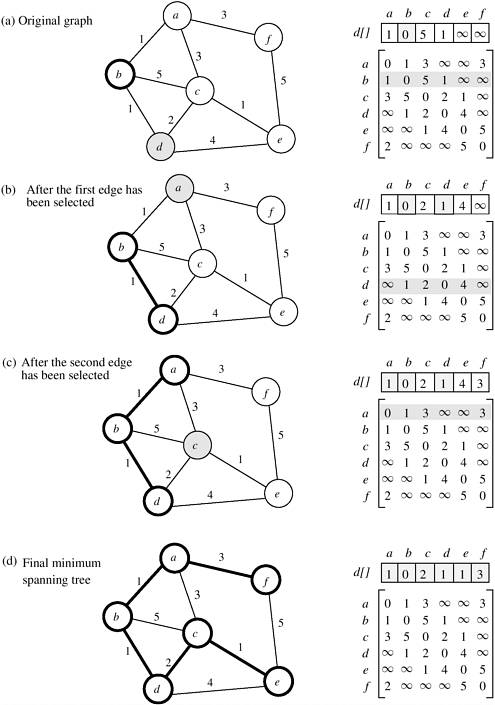
\includegraphics[width=0.75\textwidth, height=0.75\textheight,keepaspectratio]{prim.jpg}
  \caption{Minh hoạ thuật toán Prim}
\end{figure}

\clearpage

\section{Giải thuật heuristic Chèn gấn nhất - Nearest Insertion.}

Cho đến thời điểm hiện tại, lời giải nhanh và tối ưu nhất cho bài toán TSP vẫn chưa được tìm ra. Mặc dù vậy, ta có thể tìm ra được lời giải \textit{tạm chấp nhận được} cho bài toán một cách nhanh chóng. Một trong số các kĩ thuật để có thể tìm ra được những lời giải như vậy chính là kỹ thuật heuristic, và trong bài báo cáo này, chúng ta sẽ dùng kĩ thuật Chèn gần nhất (Nearest Insertion) để tìm một lời giải \textit{tạm chấp nhận được} cho bài toán TSP.

Nearest Insertion là kỹ thuật mở rộng đường đi, gọi là \textit{tour}, bằng cách chèn những điểm mới vào những điểm trong tour trước đó. Giải thuật này tìm những điểm nào không nằm trong tour gần nhất với bất kì điểm nào trong tour, sau đó chèn giữa hai điểm nào đó trong tour sao cho tổng trọng số trong tour là nhỏ nhất. Độ phức tạp của giải thuật này là $O(n^2)$ vì các bước tìm đỉnh và cạnh để chèn có độ phức tạp $O(n)$.

Mã giả và minh hoạ cho giải thuật Nearest Insertion được minh hoạ như hình dưới

\begin{vnalgorithm}
  \caption{Giải thuật Nearest Insertion}
  \begin{algorithmic}[1]
    \INPUT Đồ thị vô hướng, liên thông, có trọng số  $G = (V, U)$
    \OUTPUT Đường đi ngắn nhất $P$
    \STATE $P.$addTour$(k)$
    \STATE Tìm node $r$ sao cho $c_{kr}$ nhỏ nhất.
    \STATE $P.$addTour$(r)$
    \FOR {\textbf{each} $v \in V \setminus \{i, r\}$}
      \STATE Tìm node $r \notin P.V$ sao cho $c_{vr}$ nhỏ nhất.
      \STATE Tìm cạnh $(i, j) \in P.E$ sao cho $c_{ir} + c_{rj} - c{ij}$ nhỏ nhất.
      \STATE Chèn $r$ vào giữa $i$ và $j$.
    \ENDFOR
  \end{algorithmic}
\end{vnalgorithm}

\begin{figure}[h]
  \centering
  \begin{subfigure}{.3\linewidth}
      \centering
      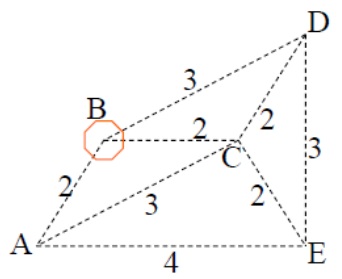
\includegraphics[width=\textwidth,height=\textheight,keepaspectratio]{ni_1.png}
      \caption{Chọn nút bất kì}
  \end{subfigure}
      \hfill
  \begin{subfigure}{.3\linewidth}
      \centering
      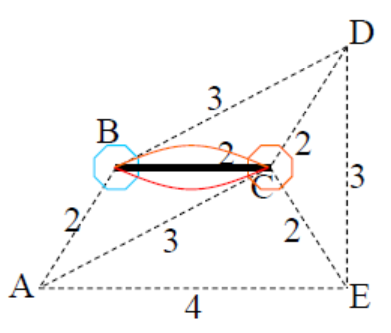
\includegraphics[width=\textwidth,height=\textheight,keepaspectratio]{ni_2.png}
      \caption{Lần lặp thứ nhất}
  \end{subfigure}
     \hfill
  \begin{subfigure}{.3\linewidth}
      \centering
      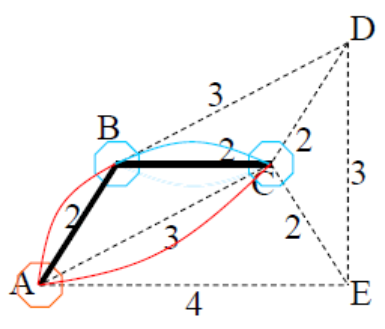
\includegraphics[width=\textwidth,height=\textheight,keepaspectratio]{ni_3.png}
      \caption{Lần lặp thứ hai}
  \end{subfigure}
  
  \bigskip
  \begin{subfigure}{.3\linewidth}
    \centering
    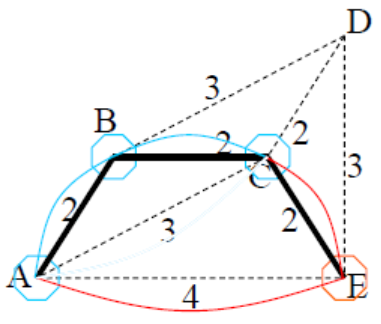
\includegraphics[width=\textwidth,height=\textheight,keepaspectratio]{ni_4.png}
    \caption{Lần lặp thứ ba}
  \end{subfigure}
  \hfill
  \begin{subfigure}{.3\linewidth}
    \centering
    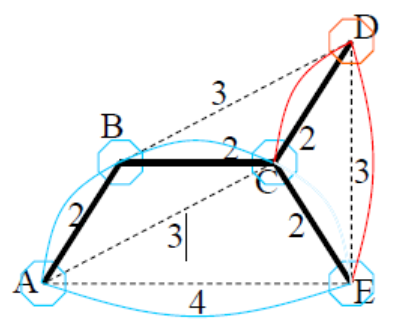
\includegraphics[width=\textwidth,height=\textheight,keepaspectratio]{ni_5.png}
    \caption{Lần lặp thứ tư}
  \end{subfigure}
  \hfill
  \begin{subfigure}{.3\linewidth}
    \centering
    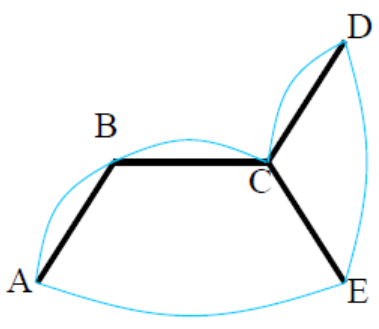
\includegraphics[width=\textwidth,height=\textheight,keepaspectratio]{ni_6.png}
    \caption{Kết quả cuối cùng}
  \end{subfigure}
  \caption{Minh hoạ giải thuật heuristic Nearest Insertion}
\end{figure}

\clearpage
\section{Kết quả trên \lstinline|Python|.}
Vận dụng thuật toán Prim và giải thuật heuristic Nearest Insertion, ta có thể cài đặt chương trình giải bài toán TSP bằng thuật toán A* trên Python 3.9.13. 

Một số hàm cần lưu ý trong chương trình gồm:

\begin{itemize}
  \item \lstinline|Graph.printMST(self, parent, g, d_temp, t)|: in ra cây khung nhỏ nhất của đồ thị và trả về trọng số của cây khung nhỏ nhất.
  \item \lstinline|Graph.minKey(self, key, mstSet)|: tìm giá trị nhỏ nhất trong tập hợp các đỉnh của cây khung nhỏ nhất.
  \item \lstinline|Graph.primMST(self, g, d_temp, t)|: thực hiện thuật toán tìm cây khung nhỏ nhất của đồ thị.
  \item \lstinline|heuristic(tree, p_id, t, V, graph)|: thực hiện giải thuật heuristic Nearest Insertion.
  \item \lstinline|checkPath(tree, toExpand, V)|: kiểm tra và in ra đường đi ngắn nhất của bài toán.
  \item \lstinline|startTSP(graph, tree, V)|: thực hiện việc giải bài toán TSP bằng thuật toán A*.
\end{itemize}

Các test case và kết quả của chương trình được minh hoạ như hình 5 và hình 6.

\begin{figure}[h]
  \centering
  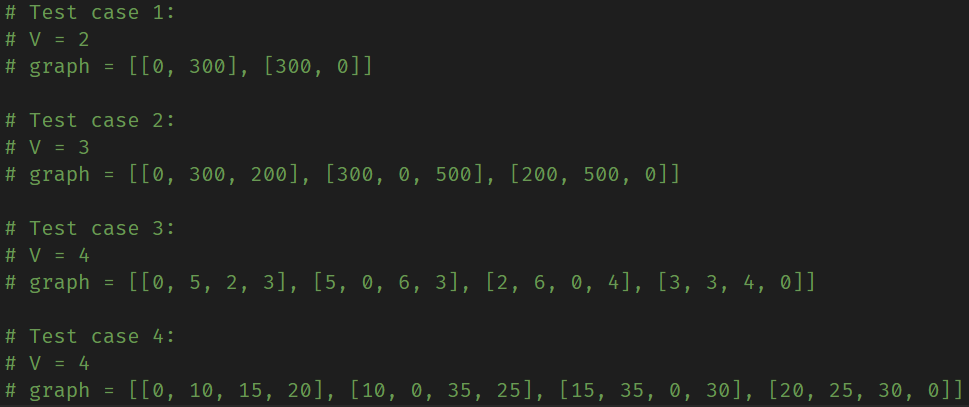
\includegraphics[width=\textwidth, height=\textheight,keepaspectratio]{test_cases.png}
  \caption{Các test case của chương trình}
\end{figure}

\begin{figure}[h]
  \centering
  \begin{subfigure}{.45\linewidth}
      \centering
      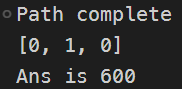
\includegraphics[width=\textwidth,height=\textheight,keepaspectratio]{res_1.png}
      \caption{Test case 1}
  \end{subfigure}
      \hfill
  \begin{subfigure}{.45\linewidth}
      \centering
      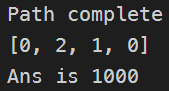
\includegraphics[width=\textwidth,height=\textheight,keepaspectratio]{res_2.png}
      \caption{Test case 2}
  \end{subfigure}
 
  \bigskip
  \begin{subfigure}{.45\linewidth}
    \centering
    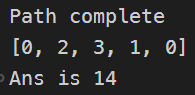
\includegraphics[width=\textwidth,height=\textheight,keepaspectratio]{res_3.png}
    \caption{Test case 3}
  \end{subfigure}
  \hfill
  \begin{subfigure}{.45\linewidth}
    \centering
    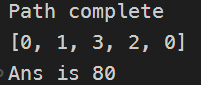
\includegraphics[width=\textwidth,height=\textheight,keepaspectratio]{res_4.png}
    \caption{Test case 4}
  \end{subfigure}
  \caption{Kết quả chạy chương trình với các test case ở hình 5}
\end{figure}


\section{Nhận xét.}
- Chương trình trên chỉ giải được khi từng cặp đỉnh trong đò thị được nối với nhau bởi 1 cạnh.

- Thuật toán trên có thể chạy chậm nếu số lượng đỉnh rất lớn.

- Ngoài giải thuật heuristic Nearest Insertion, ta có thể tối ưu lời giải bằng các giải thuật heuristic khác như giải thuật 3-Opt, giải thuật Lin-Kernighan,... 

\end{document}